\chapter{Implementation}
\label{chap:implementation}

This chapter addresses the implementation of the design detailed before. First, the technical decisions will be presented, followed by a technical view of the software developed. The next section explains how the software was tested by displaying some code examples. Finally, a brief synopsis closes this chapter.

\section{Technical Decisions}
\label{sec:implementation:decisions}

This section describes and justifies the decisions taken while developing \textbf{Sensae Console}.
As a green field project, \textbf{Sensae Console}, lacks constraints imposed by prior work, as such, all decisions have been taken during the thesis time span.

The following list unveils the most relevant technical decisions for \textbf{Sensae Console}:

\begin{itemize}
    \item \nameref{subsec:implementation:decisions:backend};
    \item \nameref{subsec:implementation:decisions:frontend};
    \item \nameref{subsec:implementation:decisions:graphql};
    \item \nameref{subsec:implementation:decisions:rabbitmq};
    \item \nameref{subsec:implementation:decisions:proto}
    \item \nameref{subsec:implementation:decisions:database};
    \item \nameref{subsec:implementation:decisions:drools};
    \item \nameref{subsec:implementation:decisions:js};
    \item \nameref{subsec:implementation:decisions:docker};
    \item \nameref{subsec:implementation:decisions:compose};
    \item \nameref{subsec:implementation:decisions:nginx};
    \item \nameref{subsec:implementation:decisions:git};
    \item \nameref{subsec:implementation:decisions:issues};
    \item \nameref{subsec:implementation:decisions:actions};
    \item \nameref{subsec:implementation:decisions:maven};
\end{itemize}

\subsection{Backend Technologies Usage throughout the Solution}
\label{subsec:implementation:decisions:backend}

The backend development is divided into three main areas:

\begin{itemize}
    \item \textit{iot-core} package;
    \item Data Flow Scope backend containers;
    \item Service and Configuration Scope backend containers (named \nameref{subsubsec:implementation:decisions:backend:geral});
\end{itemize}

In the following sub sections a brief description and justification of the technologies used is presented.

\subsubsection*{Programing Language Used}
\label{subsubsec:implementation:decisions:backend:prog}

As described in the development view of Section~\ref{subsubsec:design:architecture:context:development}, a package named \textit{iot-core}, an idealized \gls{SDK} for \textbf{Sensae Console}, was developed to define the information that flows inside the system. 
Since this project is still in the early stages, the \textit{iot-core} package was only developed in \textit{Java}.

In the future more programing languages may be supported though new \gls{SDK}s. The \textit{Rust} programing language is the next candidate due to its low memory footprint, fast startup times and expressive syntax.

The reasons that lead to the development of the first \gls{SDK} in \textit{Java} are:

\begin{itemize}
    \item It's the Programing language that the author is most familiarized with;
    \item Is widely used in industry for backend service development;
    \item Vast and robust support for virtually any technology used for backend development: database access, synchronous and asynchronous communication protocols, streaming platforms, embedded caches, rule engines and script engines.
\end{itemize}

The development of \textit{iot-core} in \textit{Java} lead to the development of all backend services also in \textit{Java}.

\subsubsection*{General Backend Services}
\label{subsubsec:implementation:decisions:backend:geral}

The services that this section encompasses can be seen as more robust and heavy due to their associated requirements.

As such, the framework used to develop them was \citetitle{springboot}, due to its vast documentation and big community. This framework comes with several modules that help to easily create stand-alone, production-grade applications. The author also had previously worked with this framework.

The main drawbacks of this framework are the slow start up time and high memory consumption, since these are not ideal for the microservices/cloud world.

\subsubsection*{Data Flow Scope Backend Services}
\label{subsubsec:implementation:decisions:backend:flow}

As discussed in Section~\ref{subsec:design:system_scopes:data_flow_scope}, the services that this section encompasses can be seen as more lightweight than the ones described above due to their associated requirements.

Since this containers process inbound device data, they have a bigger need to automatically scale. Since they need to react faster to throughput changes, their start up times must be small.

As such, the framework used to develop them was \citetitle{quarkus}. This framework has first-class support for \citetitle{graalvm}.

According to \cite{graalvm-intro}, GraalVM is a ``high-performance JDK designed to accelerate the execution of applications written in Java and other JVM languages while also providing runtimes for JavaScript, Python, and a number of other popular languages. GraalVM offers two ways to run Java applications: on the HotSpot JVM with Graal just-in-time (JIT) compiler or as an ahead-of-time (AOT) compiled native executable. GraalVM's polyglot capabilities make it possible to mix multiple programming languages in a single application while eliminating foreign language call costs.''

This features, coupled with the fact that the \textit{Quarkus} architecture follows the \citetitle{reactivemanifesto}, are appealing when compared with \citetitle{springboot} that only has experimental support for \citetitle{graalvm}, via \citetitle{spring-native}.

\subsection{Frontend Technologies Usage thought the Solution}
\label{subsec:implementation:decisions:frontend}

Even though a micro frontend architecture empowers the selection of different technologies depending on the requirements of the solution and team affinity with the stack, the Frontend Containers were developed using the same technological stack. At the time of writing there was only one developer involved, this diminished the cognitive load needed to work on the solution while still allowing future collaborators to use different frontend frameworks.

\subsubsection*{Programing Language and Framework Used}
\label{subsubsec:implementation:decisions:frontend:prog}

The author had previous contact with the following frameworks: (i) \citetitle{angular}, (ii) \citetitle{react}, and therefore no other tool was discussed when choosing the one to use in the solution.

The programming language used was \citetitle{typescript} since it is a strongly typed language and therefore leads to more robust and predictable code. Static typing helps to avoid various bugs that arise when using \citetitle{javascript}. Before transpiling \citetitle{typescript} code to \citetitle{javascript}, it is analyzed to detect bugs related to type errors.

As for the framework/library used, the following table, Table~\ref{tab:implementation:decisions:frontend:prog}, describes the reason that lead the author to choose Angular over React.

\begin{table}[H]
    \centering
    \begin{tabular}{@{}cll@{}}
    \toprule
    \textbf{Framework/Library}                                                                 & \textbf{Angular} & \textbf{React}           \\ \midrule
    \begin{tabular}[c]{@{}c@{}}Separation of User Interface\\  and Business Logic\end{tabular} & enforced         & flexible                 \\ \midrule
    Language Requirements                                                                      & typescript       & javascript or typescript \\ \midrule
    Familiarity with the tool                                                                  & high             & medium                   \\ \midrule
    \begin{tabular}[c]{@{}c@{}}UI Component Libraries with wide\\  community support\end{tabular} &
      material &
      \begin{tabular}[c]{@{}l@{}}ant design, material ui, \\ react bootstrap, semantic ui react\end{tabular} \\ \bottomrule
    \end{tabular}
    \caption{Comparison of Angular with React}
    \label{tab:implementation:decisions:frontend:prog}
\end{table}

Both tools have a wide support from the community and excellent documentation. For the author, Angular outclasses React in this project since it enforces the use of good design principles via the first and second entry described in the table above. 

\subsubsection*{Technologies used to create a Micro Frontend Architecture}
\label{subsubsec:implementation:decisions:frontend:micro}

\citetitle{modulefederation} was the tool used to seemly connect the various Frontend. No other tool was considered or researched since \textit{Angular} already relies on \textit{Webpack 5} to bundle the application and therefore it's effortless to use this tool. \citetitle{modulefederation} allows programs to reference other programs parts that are not known at compile time. In addition, the micro frontends can share libraries with each other, so that the individual bundles do not contain any duplicates.

\subsection{Expose a GraphQL API On Backend Services}
\label{subsec:implementation:decisions:graphql}

The \gls{API} discussed in this section refers to the interfaces exposed to the outside world by backend containers of the Configuration and Service Scopes and isn't related to the internal communication or device data ingestion interface exposed by the Data Relayer Container.

The two approaches considered were: (i) \citetitle{rest} and (ii) \citetitle{graphql}.

According to \cite{graphql}, ``GraphQL provides a complete and understandable description of the data in your API, gives clients the power to ask for exactly what they need and nothing more, makes it easier to evolve APIs over time, and enables powerful developer tools.''

According to \cite{rest}, ``REST APIs provide a flexible, lightweight way to integrate applications, and have emerged as the most common method for connecting components in microservices architectures.''
 
These two approaches have vast differences but they both try to answer the same question: How should one expose internal data to the outside world?

\cite{eizinger2017api}, compares these two approaches under five criteria: (i) operation reusability, (ii) discoverability, (iii) component responsibility, (iv) simplicity, (v) performance, (vi) interaction visibility and (vii) customizability.

\citetitle{graphql} was the chosen approach mainly due to better operation reusability: ``The flexibility in the definition of the exactly returned data allows clients to tailor it for their specific needs, thereby achieving highly reusable data retrieval operations.'' and interaction visibility: ``With GraphQL featuring a declarative language, intermediaries capable of understanding the GraphQL grammar can at least partly reason about the communication between a client and a GraphQL server.''

\cite{eizinger2017api}, when discussing the complexity of each approaches also highlights that ``GraphQL makes fetching data in various ways really simple for the client.''

The idea behind the highly decoupled architecture of this solution derives from the need to provide knowledgeable customers with the tools to easily design and incorporate their solutions in \textbf{Sensae Console}. The usage of \citetitle{graphql} further complements this idea by providing an API that is simple to understand and consume.

\subsection{Usage of RabbitMQ to support Internal Communication}
\label{subsec:implementation:decisions:rabbitmq}

As discussed in Section~\ref{subsec:design:alternatives:internal} and \ref{subsec:design:alternatives:flow}, the technology ultimately chosen was for internal communication was \citetitle{rabbitmq}. This message broker was chosen in detriment of others since the author had previously worked with the technology.

As discussed in the article, \citetitle{rabbitmqexpl}, the \gls{AMQP} 0.9.1 protocol defines four main concepts: (i) publisher, (ii) exchange, (iii) queue, (iv) consumer. The following diagram, Figure~\ref{fig:implementation:decisions:rabbitmq} explains how this concepts interact.

\begin{figure}[H]
    \centering
    \resizebox{\columnwidth}{!}
    {
       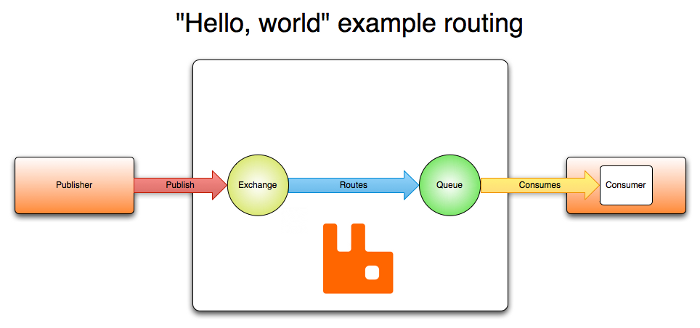
\includegraphics{assets/figures/rabbitmq.png}
    }
    \caption[\gls{AMQP} 0.9.1 Protocol Concepts]{\gls{AMQP} 0.9.1 Protocol Concepts by \cite{rabbitmqexpl}}
    \label{fig:implementation:decisions:rabbitmq}
 \end{figure}

As discussed in \citetitle{rabbitmqexpl}, there are four types of exchanges: 

\begin{itemize}
    \item Direct Exchange: ideal for the unicast routing of messages;
    \item Fanout Exchange: ideal for the broadcast routing of messages;
    \item Topic Exchange: ideal for the multicast routing of messages, queues subscribe to specific routing keys;
    \item Header Exchange: ideal for more flexible unicast routing of messages, queues subscribe to specific message headers;
\end{itemize}

The exchange that better fits the defined requirements is the Topic Exchange.

When working with this protocol and type of exchange, some drawbacks were found:

When dealing with Topic Exchanges a Consumer can only subscribe to one specific routing key or all at once - via \textit{*}- this makes it complex to create routing keys with dynamic values. As an example, lets look at the \textit{Channel} routing key defined in Table~\ref{tab:design:domain:shared_model:routing} of Section~\ref{subsubsec:design:domain:shared_model:routing}. This key defines the single destination of a data unit. For a data unit to have various dynamic service destinations there would be a need to either:

\begin{itemize}
    \item Ensure that every single service subscribes to all relevant combinations of \textit{channel}s possible, deemed impractical;
    \item Duplicate data units, where each copy would be assigned a different channel, deemed inefficient;
\end{itemize}

To tackle this issue, another Message Broker, such as \citetitle{pulsar}, with its own protocol, can be used in the future. This Message Broker answers the drawback describe above by allowing Consumers to subscribe to multiple topics (equivalent to RabbitMQ' routing keys) on the basis of a regular expression (regex), as stated in \citetitle{pulsarmulti}.

The other drawback found is that, according to the \citetitle{rabbitmqprotocol} the routing keys have a max size of 255 bytes. As described in Table~\ref{tab:design:domain:shared_model:routing} of Section~\ref{subsubsec:design:domain:shared_model:routing}, the system currently supports various keys and more keys are expected to be added in the future, meaning that this cap may one day be reached. This limitation lead to the encoding of routing keys in a single character when possible.

\subsection{Usage of Protocol Buffers in Internal Communication}
\label{subsec:implementation:decisions:proto}

This section refers to how messages that flow in the system (via Message Broker) are serialized and deserialized. The common formats used to send structured data across systems are \gls{JSON} and \gls{XML}. This formats, when compared with \citetitle{proto} or \citetitle{thrift}, sacrifice size and de/serialization performance for human readability as stated in \cite{sumaray2012comparison}.

As mentioned before, \textbf{Sensae Console} aims to provide a good developer experience for external costumers that want to expand the solution according to their needs. Due to this, the final decision weighted heavily on formats that were self-documented, e.g. defined by a strict \textit{data schema}, such as \citetitle{proto} and \citetitle{thrift}.

This two technologies, \citetitle{proto} and \citetitle{thrift}, have similar goals and approaches to the problem they try to solve. They both rely on code generation based on a schema of the data structure. The tools related to this formats officially support various languages such as \textit{Java}, \textit{C++}, \textit{C\#}, \textit{Python}, \textit{Go} and others. 

By leveraging this features, creating a basic \gls{SDK} in a new programing language is trivial since serialization, deserialization and data structure is already taken care by the code generation tool.

\citetitle{proto} are a ``language-neutral, platform-neutral, extensible mechanism for serializing structured data''.

\citetitle{thrift}s ``primary goal is to enable efficient and reliable communication across programming languages by abstracting the portions of each language that tend to require the most customization into a common library that is implemented in each language.''

Ultimately \citetitle{proto} were chosen due to better documentation and community support.


\subsection{Database Usage throughout the Solution}
\label{subsec:implementation:decisions:database}

This section refers to how information is stored across the system.

A \gls{DBMS} is a general-purpose software system that facilitates the processes of defining, constructing, manipulating, and sharing data - \citetitle{elmasri2000fundamentals}. \gls{DBMS}s can be categorized according to several criteria, such as the data model, number of users or number of sites. This section focus on the data model, these are some of the data model types, according to \cite{elmasri2000fundamentals}: 

\begin{itemize}
    \item The \textbf{relational data model} represents a database as a collection of tables,
    where each table can be stored as a separate file; 
    \item The \textbf{document-based data model} is based on JSON (Java Script
    Object Notation) and stores the data as documents, which somewhat resemble
    complex objects; 
    \item The \textbf{column-based data model} stores the columns of rows clustered on disk pages for fast access and allow multiple versions of the data;
    \item The \textbf{graph-based data model} stores objects as graph nodes and relationships among objects as directed graph edges;
    \item The \textbf{key-value data model} associates a unique key with each value (which can be a record or object) and provides very fast access to a value given its key.
\end{itemize}

The requirements gathered unveil the need to use three different database' data models throughout the system: (i) relational, (ii) document-based and (iii) column-based data models. The following sections answer why these data models were needed and what technologies were chosen for each of them. A final section unveils an optional solution that was considered but ultimately not pursued.

\subsubsection*{Relational Database Usage}
\label{subsubsec:implementation:decisions:database:relational}

This data model has a wide variety of usage in the industry. Some of the technologies that follow this data model are: (i) \citetitle{mysql}, (ii) \citetitle{postgressql} and (iii) \citetitle{mariadb}.

It is intended for strictly structured data with well defined interrelations. This type of data can be found on most Bounded Contexts described in Section~\ref{subsec:design:domain:bounded_contexts} such as \nameref{subsubsec:design:domain:bounded_contexts:processor}, \nameref{subsubsec:design:domain:bounded_contexts:decoder}, \nameref{subsubsec:design:domain:bounded_contexts:device}, \nameref{subsubsec:design:domain:bounded_contexts:identity}, \nameref{subsubsec:design:domain:bounded_contexts:rule} and the Irrigation Zone/Device concepts of the \nameref{subsubsec:design:domain:bounded_contexts:irrigation} Context.

As such, this data model was adopted for the \textbf{Device Management Database}, \textbf{Data Decoder Database}, \textbf{Data Processor Database}, \textbf{Rule Management Database}, \textbf{Identity Management Database}, \textbf{Smart Irrigation Business Database} and \textbf{Notification Management Database} containers. 

The author had previous contact with all the cited \gls{DBMS}, the decision to use \citetitle{postgressql} was taken based on the fact that, contrary to the other options, \citetitle{postgressql} supports a vast number of Data Types such as \gls{JSON}, Arrays, \gls{UUID}, and Ranges. \citetitle{postgressql}'s data model is an extension of the relation data model, named object-relational data model - \cite{elmasri2000fundamentals}. This data model supports various concepts such as objects, classes and inheritance and therefore can lead to entity models more expressive and close to the business ideas.

\subsubsection*{Document-based Database Usage}
\label{subsubsec:implementation:decisions:database:nosql}

This data model rose from the increasing need to store and analyze unstructured data as stated by \cite{miloslavskaya2016big}.  Citing \cite{elmasri2000fundamentals}, a ``major difference between document-based systems versus object and object-relational systems (...) is that there is no requirement to specify a schema''.

This type of requirements and data resembles the Data Store context described in Section~\ref{subsec:design:system_scopes:data_flow_scope} and Figures~\ref{fig:design:architecture:container:logical:diagram:data_flow} and \ref{fig:design:architecture:container:process:diagram:flow}. This context, intended to mimic a Data Lake\footnote{Massively scalable storage repository that holds a vast amount of raw data in its native format («as is») until it is needed, by \cite{miloslavskaya2016big}}, stores any type of data for future use.

As such, this data model was adopted for the \textbf{Data Store Database} container. 

The only technology considered, and therefore adopted, was \citetitle{mongodb} due to its vast community, excellent documentation and large number of libraries that ease the database management operations. \citetitle{mongodb} also supports replication and sharding according to \cite{elmasri2000fundamentals}, this features is useful once a single node isn't capable of withstanding all data collected while providing fast access to it.

\subsubsection*{Column-based Database Usage}
\label{subsubsec:implementation:decisions:database:time}

This data model is used in applications that require large amounts of data storage, and is commonly named \textit{data warehouses}. According to \cite{dehdouh2015using}, a data warehouse  is ``designed according to a dimensional modelling which has for objective to observe facts through measures, also called indicators, according to the dimensions that represent the analysis axes''. Citing \cite{han2011survey}, this databases ``can maintain high-performance of data analysis and business intelligence processing''.

This features fit the requirements related to storing and reading vast amounts of device measures. As such, it was adopter for the \textbf{Fleet Management Database} and \textbf{Smart Irrigation Data Database} containers.

The author had no previous contact with this type of data model. Some of the technologies related to this concept are: (i) \citetitle{hbase}, (ii) \citetitle{cassandradb}, (iii) \citetitle{influxdb}, (iv) \citetitle{questdb}.

According to \cite{george2011hbase} HBase is a ``distributed, persistent, strictly consistent storage system with near-optimal write and excellent read performance''. This database uses \gls{HDFS} as its file system, and so, it is built on top of Hadoop. 
HBase does not support a structured query language like \gls{SQL}, ``even though it's comprised of a set of standard tables with rows and columns, much like a traditional database'' (\cite{ibm-hbase}).

CassandraDB is a distributed storage system for managing very large amounts of structured data spread out across many commodity servers, while providing highly available service with no single point of failure (\cite{lakshman2010cassandra}).
It was developed internally by Facebook and then later open-sourced to the Apache Foundation. It doesn't support \gls{SQL}.

According to \cite{naqvi2017time}, InfluxDB is an ``open-source schemaless \gls{TSDB} with optional closed-sourced components developed by InfluxData. It is written in Go programming language and it is optimized to handle time series data.'' It provides an SQL-like query language and also defines a new protocol for fast data ingestion (\cite{ilp}).

QuestDB is a relational column-oriented database designed for time series and event data and entitles it self as the ``fastest open source time series database'' (\cite{questdb}).
According to benchmarks (\cite{quest-bench}) preformed using the \gls{TSBS}, \cite{TSBS}, QuestDB ranks as the fastest option in the market.
It has out-of-the-box support for SQL Postgres wire protocol, (thus integrating with \gls{JDBC}), can be easily deployed using a single Docker Image, and also supports the \gls{ILP}.

The type of business this solution is tackling revolves around the capture and analysis of device readings, \gls{IoT}. So the notion of time has to be treated as a first class citizen. The measurements that constitute a time series are ordered on a timeline, which reveals information about underlying patterns.

As stated by \cite{naqvi2017time}, \gls{TSDB} ``can be used to efficiently store sensors and devices' data'' since, ``such technologies are generating large amount of data which is usually time-stamped''.

With this requirements in hand, a column-based data model isn't enough. The technology adopted should also natively support time series to ease data analysis. As such, the \citetitle{hbase} and \citetitle{cassandradb} options were discarded.

Between the two missing options, the author picked \citetitle{questdb} due to better support for \gls{SQL} though \gls{JDBC}. During the research of this two technologies no major downside was found for \citetitle{questdb} when compared to \citetitle{influxdb}.

\subsubsection*{Graph-based Database Usage}
\label{subsubsec:implementation:decisions:database:identity}

Even tho this data model was ultimately not used, the author deemed relevant to mention it.

As stated in the bounded context's section of~\nameref{subsubsec:design:domain:bounded_contexts:identity}, the domains follow a hierarchical structure that can resemble a graph. This context in particular would benefit from a  graph-based database, but this option was not pursued since the author had no previous contact with this family of technologies. Instead \citetitle{postgressql} was used.

\citetitle{postgressql} can represent logical hierarchical structures and concepts using the array data type as the \textit{path} from the root domain to the current domain.

Queries that revolve around graph concepts such as: select parent node, select child nodes, move nodes to a new parent and others, can be preformed efficiently using array operators such as \textbf{\&\&}, \textbf{||} and \textbf{@>}\footnote{taken from PostgresSQL Documentation: \citetitle{postgresarray} \& \citetitle{postgresarrayop}}.

\subsection{Rules Script Engine}
\label{subsec:implementation:decisions:drools}

This section refers to the bounded context of \textbf{Rule Management}. As mentioned before, the purpose of this context is to provide a high-level language that can analyze a stream of Data Units and output alerts base on them. The technology adopted was \citetitle{drools}.

\citetitle{drools} is an open-source rule engine widely used in the industry. The features that stud out from other rule engines were:

\begin{itemize}
    \item Supports for sliding windows of time;
    \item Is also a \gls{CEP} System;
    \item Integrates with the \textit{iot-core} package since it is also written in \textit{Java};
    \item Can be used as a standalone application or an embedded component of another application;
    \item Has an expressive, yet complex, syntax to write rules; 
    \item Can dynamically load rules at runtime.
\end{itemize}

The Section~\ref{subsec:implementation:description:rule} details how one can write rule scenarios.

\subsection{Data Decoders Script Engine}
\label{subsec:implementation:decisions:js}

This section refers to the bounded context of \textbf{Data Decoder}. As mentioned before, this context purpose is to translate inbound Data Units into a format and semantics that the system can understand. The technology adopted was \textit{Javascript}.

\textit{Javascript} is a high level language with an enormous community and is widely used in the industry. Another big reason behind this decision is that a lot of companies producing \gls{IoT} devices provide open-source decoders written in \textit{Javascript}, such as \href{https://github.com/Milesight-IoT/SensorDecoders}{Milesight}
\footnote{\href {https://github.com/Milesight-IoT/SensorDecoders}{github.com/Milesight-IoT/SensorDecoders}}, \href{https://github.com/SensationalSystems}{SensationalSystems}, \href{https://github.com/helium/console-decoders}{Helium}, 
\footnote{\href {https://github.com/helium/console-decoders}{github.com/helium/console-decoders}} and
\footnote{\href {https://github.com/SensationalSystems}{github.com/SensationalSystems}}. This makes it easy and straightforward to integrate new decoders in \textbf{Sensae Console}.

The Section~\ref{subsec:implementation:description:decoder} details how one can write decoders.

\subsection{Containerization of services via Docker}
\label{subsec:implementation:decisions:docker}

This section describes how the final product is packaged using \citetitle{docker}.

As stated in \citetitle{dockerinit}, Docker acts as an intermediary layer between the application to be deployed and the operating system where it will be deployed, ensuring that the developed software has the same behavior regardless of the system. The dependencies of the solution do not have to be present in the system, it is only necessary to install the Docker tool in the \gls{OS}.

This tool thus makes it possible to lower the coupling between the \gls{OS} and the software to be deployed.

With regards for this solution, each container defined in Section~\ref{subsec:design:architecture:containers} is mapped into a docker container.
A container is often compared to a virtual machine running on a hypervisor or
\gls{OS}, but it has a much lower resource consumption, since only the application is run and not not all the processes inherent to an \gls{OS}. Containers execute calls directly to the kernel running on the physical machine and can be seen, unlike virtual machines with their own kernel, as a normal process.

The system is thus represented as a collection of containers that communicate with each other and the outside through standard protocols such as HTTP or AMQP.

The production environment can thus be quickly replicated on another machine in case of a failure disaster or a overwhelming number of interaction with the server.

\subsection{Orchestration of services via Docker Compose}
\label{subsec:implementation:decisions:compose}

This section describes how the final product is orchestrated using Docker Compose.

As stated in the article \citetitle{dockercompose}, ``Compose is a tool for defining and running multi-container Docker applications''. 

Since there is no need to automatically scale the solution it was decided to use a docker compose in production inserted of tools like Kubernetes.

The solution's orchestration is defined in a \textit{YAML} file and then started with a single command. To improve security, only the needed container ports are exposed. To ensure data integrity throughout service disruptions, persistence data is mapped to folder in the \gls{OS}. To ensure an easy management of the environment, configurations are kept in the \gls{OS} and fetched by each container once they start. 

\subsection{Usage of Nginx as a web server and reverse proxy}
\label{subsec:implementation:decisions:nginx}

To serve the frontend pages and redirect requests made to backend containers, the following technologies were analyzed:

\begin{itemize}
    \item \citetitle{nginx};
    \item \citetitle{apachehttp};
    \item \citetitle{lighttpd};
\end{itemize}

All of them support the necessary requirements, but some factors lead the author to pick Nginx over the others, the following table, Table~\ref{tab:implementation:decisions:nginx:compare}, describes this criteria.

\begin{table}[H]
    \centering
    \begin{tabular}{@{}clll@{}}
    \toprule
    \textbf{Criteria/Technology} & \textbf{Nginx} & \textbf{Apache HTTP Server} & \textbf{Lighttpd} \\ \midrule
    Resource Consumption      & low  & high      & medium \\ \midrule
    Community Size            & high & very high & medium \\ \midrule
    Familiarity with the tool & high & low       & low    \\ \bottomrule
    \end{tabular}
    \caption{Technologies Comparison - Reverse Proxy Web Server }
    \label{tab:implementation:decisions:nginx:compare}
\end{table}

\subsection{Usage of Git as a version control system of the project}
\label{subsec:implementation:decisions:git}

\citetitle{git} is a \gls{VCS}. What differentiates it from other
systems such as \citetitle{mercurial} and \citetitle{bitkeeper} is its branching model. It is currently also the most widely used.

\citetitle{github} was the platform used to host the developed code. It offers private repositories with no additional costs. This platform also has other tools such as \textit{Github Issues} and \textit{Github Actions} that ease a developer's workflow. 

A \gls{VCS} is indispensable in software development, this system allows developers to store the history of changes made to the code in an organized manner and simplifies the management of the software by the development team. This system was chosen over others because of the author was experienced with this software.

The development of the entire solution was made in two separated repositories, one for \textit{iot-core} and another for \textbf{Sensae Console}.

The \textit{iot-core} repository had a simple branching model consisting only of a master branch. 

There was an extensive use of the branching feature in the repository of \textbf{Sensae Console}, following the model shown in Figure~\ref{fig:implementation:decisions:git:branch}. The author settled for the following: a master branch that matches the deployed version, a development branch where the various features are introduced until a new version is published on the master branch, several branches dedicated to fixing bugs (hotfix) and another several branches that introduce new features and improvements (feature \textit{x}).

\begin{figure}[H]
    \centering
    \resizebox{\columnwidth}{!}
    {
       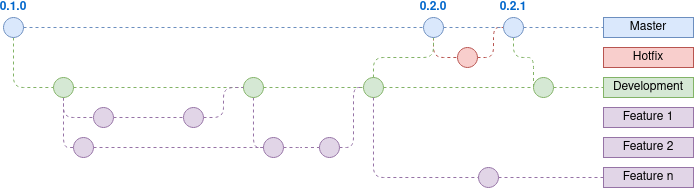
\includegraphics{assets/figures/branching-model.png}
    }
    \caption[Branching Model]{Branching Model}
    \label{fig:implementation:decisions:git:branch}
\end{figure}

This model was adopted since the project was in an initial phase of development, in the future, a branching model with multiple releases, as detailed in Figure~\ref{fig:implementation:decisions:git:branch2}, is preferred. With this model one can release only the altered containers and not the entire system.

\begin{figure}[H]
    \centering
    \resizebox{\columnwidth}{!}
    {
       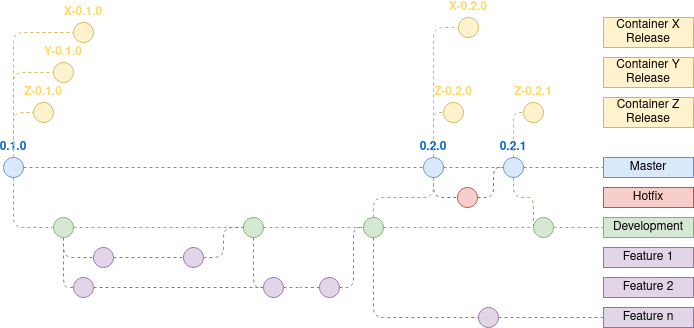
\includegraphics{assets/figures/branching-model-2.png}
    }
    \caption[Future Branching Model]{Future Branching Model}
    \label{fig:implementation:decisions:git:branch2}
\end{figure}

This is useful when using CI/CD pipelines to compile, package and deploy the various containers of the solution. If no changes have been made to \textit{X} Container there is no need to redo all the work previously done with it.

\subsection{Usage of Github Issues to track issues, bugs and new features}
\label{subsec:implementation:decisions:issues}

As described before, the code is hosted in \citetitle{github}. One of the services that this platform offers is \textit{Github Issues}. This tool helps to track and document the development process alongside with the code.

This tool can be separated into two main views. A view is concerned about what issues, features and bugs are active in the project, Figure~\ref{fig:implementation:decisions:issues:board}, and the other is concerned with the current state of each issue, feature and bug, Figure~\ref{fig:implementation:decisions:issues:project}.

\begin{figure}[H]
    \centering
    \resizebox{\columnwidth}{!}
    {
       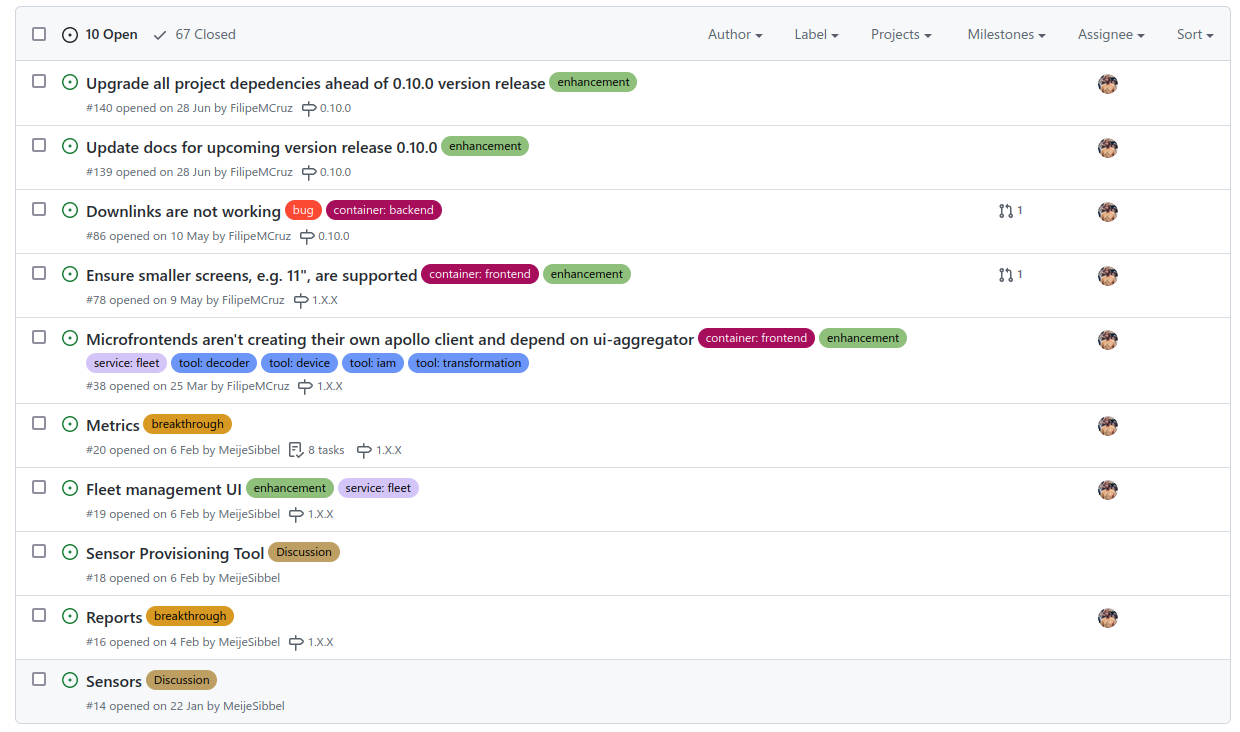
\includegraphics{assets/figures/github-2.png}
    }
    \caption[Github Issues]{Github Issues}
    \label{fig:implementation:decisions:issues:board}
\end{figure}

Each issue has a list of tags that represent its scope and a defined milestone. With this tool, the team members can also discuss issues in depth. 

The issues presented in this page are then tracked in the \textit{project} page - Figure~\ref{fig:implementation:decisions:issues:project}. The author decided to divided the issues into 4 criteria:

\begin{itemize}
    \item \textbf{To Do}: Issues that have been discussed and are to be completed in the near future; 
    \item \textbf{In Progress}: Issues that are currently under development and have an assigned feature branches;
    \item \textbf{Done}: Issues that have been completed and have been integrated in the \textit{master} branch; 
    \item \textbf{Future}: Issues that have been purposed but have no clear deadline.
\end{itemize}

\begin{figure}[H]
    \centering
    \resizebox{\columnwidth}{!}
    {
       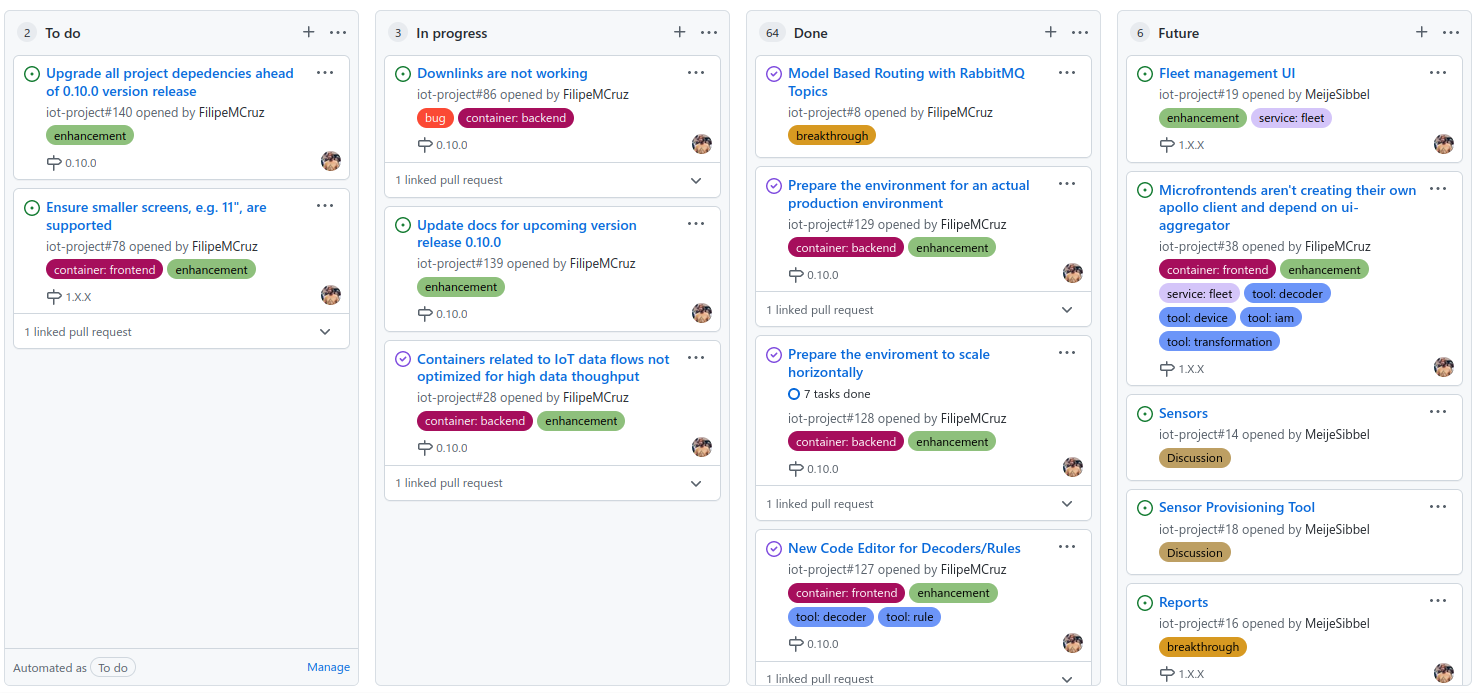
\includegraphics{assets/figures/github.png}
    }
    \caption[Github Issues Project Board]{Github Issues Project Board}
    \label{fig:implementation:decisions:issues:project}
\end{figure}

This view helps to define a simple project roadmap and track the overall state of issues, bugs and features in the project.

\subsection{Usage of Github Actions for CI/CD}
\label{subsec:implementation:decisions:actions}

Since the code is hosted in \textit{Github}, it was decided to leverage the CI/CD features of the platform. \textit{Github Actions} purpose is to automate software workflows via CI/CD.

According to \cite{cicd}, the term CI/CD represents a method to delivering applications to clients by introducing automation into the development states.
It is divided into three concepts:

\begin{itemize}
    \item \textbf{Continuous Integration}: new versions of the project are regularly submitted, tested and merged into the current project;
    \item \textbf{Continuous Delivery}: new versions of the project are automatically archived in a repository where they can then be deployed to a production environment;
    \item \textbf{Continuous Deployment}: new versions of the project are automatically deployed to a production environment.
\end{itemize}

The \textit{iot-core} package is archived in a repository so that it can then be integrated in the backend containers of \textbf{Sensae Console}, and possibly in other projects. To do so, the team uses \textit{Github Actions}. This tool's behavior is defined in a YAML file, presented in the Code Sample~\ref{code:implementation:decisions:actions:iotcore}.

\begin{lstlisting}[style=yaml, caption=Configuration File for \textit{iot-core} Continuous Delivery, label={code:implementation:decisions:actions:iotcore}]
name: IoT Core - Continuous Delivery to maven central
on:
  push:
    tags:        
      - '**'
      - '*'
jobs:
  build:
    runs-on: ubuntu-latest
    steps:
      - uses: actions/checkout@v2
      - name: Set up Maven Central Repository
        uses: actions/setup-java@v1
        with:
          java-version: 17
          server-id: ossrh
          server-username: MAVEN_USERNAME
          server-password: MAVEN_PASSWORD
          gpg-private-key: ${{ secrets.MAVEN_GPG_PRIVATE_KEY }}
          gpg-passphrase: MAVEN_GPG_PASSPHRASE
      - name: Deploy with Maven
        run: mvn -B clean deploy -Pci-cd
        env:
          MAVEN_USERNAME: ${{ secrets.OSSRH_USERNAME }}
          MAVEN_PASSWORD: ${{ secrets.OSSRH_TOKEN }}
          MAVEN_GPG_PASSPHRASE: ${{ secrets.MAVEN_GPG_PASSPHRASE }}
\end{lstlisting}

As we can see in lines \textbf{2} to \textbf{6}, this action is triggered every time a new git tag is pushed to the repository.
This action then procedes to download and setup java and maven - lines \textbf{12} to \textbf{20}. Finally it runs a maven command to deploy the new version to the artifact repository - lines \textbf{21} to \textbf{26}. 

The \textbf{Sensae Console} has an action to deal with Continuous Integration - Code Sample~\ref{code:implementation:decisions:actions:cisensae}, where changes made to the software are tested.

\begin{lstlisting}[style=yaml, caption=Configuration File for \textbf{Sensae Console} Continuous Integration, label={code:implementation:decisions:actions:cisensae}]
name: Sensae Console - Continuous Integration - Test changes 
on:
  push:
  branches:
    - master
    - dev
jobs:
  build:
    runs-on: ubuntu-latest
    steps:
      - uses: actions/checkout@v3
      - name: Set up JDK 17
        uses: actions/setup-java@v3
        with:
          java-version: "17"
          distribution: "adopt"
      - name: Test with Maven
          run: ./project/script/run-backend-tests.sh
\end{lstlisting}

As we can see in lines \textbf{2} to \textbf{6}, this action is triggered every time a new commit is push to the \textit{dev} and \textit{master} branches.
This action then procedes to download and setup java and maven - lines \textbf{10} to \textbf{16}. Finally it runs a script that tests the backend services - line \textbf{18}.

The mentioned script has the following structure - Code Sample~\ref{code:implementation:decisions:actions:testscript}.

\begin{lstlisting}[caption=Backend services test script, label={code:implementation:decisions:actions:testscript}]
#!/usr/bin/sh

ROOT_DIR=$(git rev-parse --show-toplevel)

cd "$ROOT_DIR"/project/backend-services || exit

rm --f -- ../test-examples/backend-test-pass.log
rm --f -- ../test-examples/backend-test-fail.log

ls -I data-relayer | xargs -I % sh -c 'cd % && mvn test && \
    echo % >> ../../test-examples/backend-test-pass.log || \
    echo % >> ../../test-examples/backend-test-fail.log'

test ! -f ./../test-examples/backend-test-fail.log    
\end{lstlisting}

This script runs the command \textit{mvn test} for all backend containers and stores the results of each container in a file - lines \textbf{13} to \textbf{15}. In the end, the script checks if any container didn't pass the tests - line \textbf{15} - and exists correspondingly.

\subsection{Usage of Maven Repository to host Open-Source Code}
\label{subsec:implementation:decisions:maven}

As stated in the previous section \textit{iot-core} is delivered to an artifact repository. Since the intent of this package is to be used by any one interested on integrating his/her tool with \textbf{Sensae Console}, the artifact repository has to be publicly available. 

The Maven Central repository was the chosen one, since the \textit{maven} and \textit{gradle} tools use it, by default, to fetch dependencies.

According to the article \citetitle{centralreq} by \cite{centralreq}, to publish an artifact to maven central, a couple of additions have to be made in the \textit{pom.xml} of the project namely: (i) Supply Javadoc and Sources, (ii) Provide Files Checksums, (iii) Sign Files with GPG/PGP, (iv) Sufficient Metadata, (v) Correct Coordinates, (vi) Project Name, Description and URL, (vii) License Information, (vii) Developer Information, (viii) SCM Information.

In the \refname{***TODO***} Appendix the full \textit{pom.xml} is presented.

\section{Technical Description}
\label{sec:implementation:description}

\subsection{Description of Sensae Console UI}
\label{subsec:implementation:description:ui}

\subsection{Description of Sensae Console API}
\label{subsec:implementation:description:api}

\subsection{Description of Sensae Console Data Ingestion Endpoint}
\label{subsec:implementation:description:ingestion}

\subsection{Description of Sensae Console Rule Engine}
\label{subsec:implementation:description:rule}

\subsection{Description of Sensae Console Data Decoders}
\label{subsec:implementation:description:decoder}

\subsection{Description of Configuration Files}
\label{subsec:implementation:description:config}

\section{Testing}
\label{sec:implementation:testing}

\subsection{Unit Tests}
\label{subsec:implementation:tests:unit}

\subsection{Integration Tests}
\label{subsec:implementation:tests:integration}

\subsection{Functional Tests}
\label{subsec:implementation:tests:functional}

\subsection{End-to-End Tests}
\label{subsec:implementation:tests:endtoend}

\subsection{Architectural Tests}
\label{subsec:implementation:tests:arch}

\subsection{Performance Tests}
\label{subsec:implementation:tests:performance}

\section{Synopsis}
\label{sec:implementation:synopsis}
